% SPDX-License-Identifier: CC-BY-SA-4.0
% Part: Introduction
% Section: Mathematical and Logical recalls
% Challenge exercise: Foundation of inductive definitions

\begingroup

\begin{exercice}[Mini-défi -- Définition inductive]\label{exo:introduction/maths/challenge}

  On cherche à définir formellement le sous-ensemble $E$ de $\mathbb{R}$ représenté graphiquement ci-dessous: 
  \begin{center}
    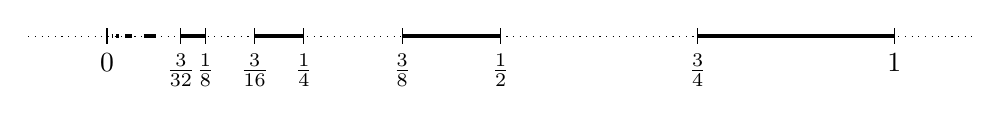
\begin{tikzpicture}
      \draw[dotted] (-1,1) -- (11,1);
      \draw[ultra thick] (7.5/1  ,1) -- (10/1  ,1);
      \draw[ultra thick] (7.5/2  ,1) -- (10/2  ,1);
      \draw[ultra thick] (7.5/4  ,1) -- (10/4  ,1);
      \draw[ultra thick] (7.5/8  ,1) -- (10/8  ,1);
      \draw[ultra thick] (7.5/16 ,1) -- (10/16 ,1);
      \draw[ultra thick] (7.5/32 ,1) -- (10/32 ,1);
      \draw[ultra thick] (7.5/64 ,1) -- (10/64 ,1);
      \draw[ultra thick] (7.5/128,1) -- (10/128,1);

      \draw (0    ,1.1) -- (0    ,0.9) node[below]{$0$};
      \draw (7.5/8,1.1) -- (7.5/8,0.9) node[below]{$\frac{3}{32}$};
      \draw (1.25 ,1.1) -- (1.25 ,0.9) node[below]{$\frac{1}{8}$};
      \draw (7.5/4,1.1) -- (7.5/4,0.9) node[below]{$\frac{3}{16}$};
      \draw (2.5  ,1.1) -- (2.5  ,0.9) node[below]{$\frac{1}{4}$};
      \draw (7.5/2,1.1) -- (7.5/2,0.9) node[below]{$\frac{3}{8}$};
      \draw (5    ,1.1) -- (5    ,0.9) node[below]{$\frac{1}{2}$};
      \draw (7.5  ,1.1) -- (7.5  ,0.9) node[below]{$\frac{3}{4}$};
      \draw (10   ,1.1) -- (10   ,0.9) node[below]{$1$};
    \end{tikzpicture}
  \end{center}

  On commence par remarquer que $E$ vérifie l'équation (\ref{equation:introduction/maths/inductive_defs}) ci-dessous :
  \begin{equation}\label{equation:introduction/maths/inductive_defs}
    \left[\frac{3}{4} , 1\right] \subseteq E
    \quad\land\quad
    \forall x \in E,  \frac{x}{2} \in E
  \end{equation}
    
  Soit $\displaystyle \mathcal{S} \eqdef \left\{X\in \mathscr{P}(\mathbb{R}) \,\middle|\, \left[\frac{3}{4} , 1\right] \subseteq X \land \forall x \in X, \frac{x}{2} \in X\right\} $
  l'ensemble des solutions de l'équation (\ref{equation:introduction/maths/inductive_defs}). 
  
  \begin{question}
  \item Montrer que $\mathbb{R} \in \mathcal{S}$, $[0, 1] \in \mathcal{S}$ et $\left[0, \frac{1}{2}\right] \cup \left[\frac{3}{4} , 1\right] \in \mathcal{S}$.
  \item Montrer que $\forall X \in \mathcal{S}, \forall X' \in \mathcal{S}, X \cap X' \in \mathcal{S}$.
  \end{question}

  On définit $E$ comme la plus petite des solutions au sens de l'inclusion :
  $$E \eqdef \bigcap_{X\in \mathcal{S}} X = \{x \in \mathbb{R} \mid \forall X \in \mathcal{S}, x \in X\}.$$

  \begin{question}
  \item Montrer que $1 \in E$ et que $\frac{1}{2} \in E$.
  \item Montrer que $2 \notin E$ et que $\frac{2}{3} \notin E$.
  \item Montrer que $\forall x < 1, x\notin E \Rightarrow \frac{x}{2} \notin E$.
    %  \item Montrer que $\forall X \in \mathscr{P}(\mathbb{R}), ([\frac{3}{4}, 1] \subseteq X \land \forall x \in X, \frac{x}{2} \in X) \implies E \subseteq X$
  \end{question}

  On pose maintenant le prédicat suivant : $P(x) \eqdef \exists y \in \mathbb{R}, 0 < y < x \land  y\notin E$.\\
  On cherche à démontrer $\forall x\in E, P(x)$ \emph{par induction sur $x$}.
  \begin{question}
  \item Montrer que $\forall x \in \left[\frac{3}{4}, 1\right], P(x)$.
  \item Montrer que $\forall x \in E, P(x) \Rightarrow P\left(\frac{x}{2}\right)$.
  \item Montrer que $\forall x\in E, P(x)$.
  \end{question}

\end{exercice}

\endgroup
\endinput
